\documentclass[12pt,a4paper]{article}

% --- Paquetes base (orden recomendado) ---
\usepackage[spanish,es-noshorthands]{babel} % <-- evita conflictos con TikZ
\usepackage[utf8]{inputenc}                 % Con Xe/LuaLaTeX puedes omitirla
\usepackage[T1]{fontenc}
\usepackage{lmodern}                        % Fuentes escalables
\usepackage{microtype}   



\usepackage{geometry}
\geometry{margin=2.5cm}
\usepackage{setspace}         % Interlineado 1,15
\usepackage{ragged2e}         % \justifying
\usepackage{fancyhdr}         % Encabezados/pies de página
\usepackage{hyperref}
\hypersetup{colorlinks=false}

% --- Tablas y columnas anchas ---
\usepackage{booktabs}
\usepackage{tabularx}
\usepackage{array}
\usepackage{makecell}
\usepackage[table]{xcolor}
\usepackage[section]{placeins} % fuerza a que los floats no crucen secciones


\newcolumntype{Y}{>{\RaggedRight\arraybackslash}X}

% --- Diagramas ---
\usepackage{tikz}
\usetikzlibrary{arrows.meta,positioning,babel,fit,shapes.symbols, calc}
\definecolor{becaccent}{HTML}{E84E36} % color acento (tú lo puedes cambiar)
\tikzset{
  block/.style={draw, rounded corners, align=center, minimum height=10mm, minimum width=32mm, inner sep=3pt},
}

% --- Imágenes y figuras
\usepackage{graphicx}     % incluir imágenes
\usepackage{caption}      % controlar estilo de leyendas (opcional)
\usepackage{float}        % para usar [H] (opcional)
\graphicspath{{figuras/}} % ruta por defecto para las imágenes (opcional)


% --- Estilo de página: número centrado abajo ---
\pagestyle{fancy}
\fancyhf{}
\cfoot{\thepage}
\renewcommand{\headrulewidth}{0pt}
\renewcommand{\footrulewidth}{0pt}

% --- Datos de portada ---
\newcommand{\Universidad}{Universidad Andrés Bello}
\newcommand{\Materia}{Tecnologías Disruptivas}
\newcommand{\NRC}{8090}
\newcommand{\Profesor}{Álvaro Sánchez Colmenares}
\newcommand{\NombreCaso}{Estudio de Caso BEC}

% Integrantes ordenados por apellido + correos
\newcommand{\Integrantes}{%
  \begin{tabular}{@{}l}
    \textbf{Gabriel Cuevas}\\[-2pt]
    \texttt{\href{mailto:g.cuevasortzar@uandresbello.edu}{g.cuevasortzar@uandresbello.edu}}\\[6pt]
    \textbf{Alfredo Fuentes}\\[-2pt]
    \texttt{\href{mailto:a.fuentesnavarrete@uandresbello.edu}{a.fuentesnavarrete@uandresbello.edu}}\\[6pt]
    \textbf{Felipe Ochoa}\\[-2pt]
    \texttt{\href{mailto:f.ochoajohn@uandresbello.edu}{f.ochoajohn@uandresbello.edu}}\\[6pt]
    \textbf{Alonso Rodrigo Urra Villagra}\\[-2pt]
    \texttt{\href{mailto:a.urravillagra@uandresbello.edu}{a.urravillagra@uandresbello.edu}}\\[6pt]
    \textbf{Antonia Valdebenito}\\[-2pt]
    \texttt{\href{mailto:a.valdebenitofuentes@uandresbello.edu}{a.valdebenitofuentes@uandresbello.edu}}
  \end{tabular}
}

\newcommand{\Fecha}{\today}

\begin{document}

% --- Portada (sin número) ---
\pagenumbering{gobble}
\begin{titlepage}
  \centering
  \vspace*{1cm}
  {\Large \Universidad\par}
  \vspace{3cm}
  {\LARGE\bfseries \NombreCaso\par}
  \vspace{1.5cm}
  {\large \Materia\ (\textbf{NRC:} \NRC)\par}
  \vspace{0.4cm}
  {\large \textbf{Profesor a cargo:} \Profesor\par}
  \vspace{2.2cm}
  {\large \textbf{Integrantes}\par}
  \vspace{0.3cm}
  {\large \Integrantes\par}
  \vfill
  {\large \Fecha\par}
\end{titlepage}

% --- Cuerpo del informe ---
\clearpage
\pagenumbering{arabic}  % Numeración desde aquí
\setstretch{1.15}       % Interlineado 1,15
\justifying             % Texto justificado

\section*{Contexto del caso — Seguridad}

La ciudad ficticia \textit{Nueva Aurora} enfrenta un rápido crecimiento poblacional y se encuentra en un proceso de transformación hacia una \textit{Smart City}. En el eje de seguridad ciudadana, el desafío principal se manifiesta en el aumento de robos y en la baja integración de cámaras y sensores a nivel urbano, situación que limita la prevención, la reacción oportuna y la trazabilidad de incidentes.

Ante este contexto, la ciudad evalúa la adopción de tecnologías propias de las ciudades inteligentes —entre ellas, Internet de las Cosas (IoT), Inteligencia Artificial (IA), Big Data, \textit{blockchain}, 5G y soluciones energéticas asociadas— como base para articular un ecosistema de seguridad más proactivo, interoperable y basado en datos. Estas capacidades tecnológicas se consideran habilitadoras para la detección temprana de eventos, la coordinación táctica y la rendición de cuentas, con énfasis en el uso de IA en cámaras urbanas y el despliegue de sensores distribuidos.

\section{Definición del problema y alcance}

\subsection*{Problemas prioritarios (resumen)}
\textbf{P1. Robos en espacio público y comercio de alta afluencia.} La ciudad evidencia un aumento sostenido de delitos contra la propiedad en zonas céntricas y nodos de transporte, afectando a peatones y locales comerciales.

\textbf{P2. Baja integración operativa de cámaras y sensores urbanos.} La infraestructura de videovigilancia y sensorización existe de forma fragmentada, sin interoperabilidad suficiente para detección temprana, trazabilidad ni coordinación de respuesta.

\subsection*{Causas principales}
\begin{itemize}
    \item \textit{Fragmentación tecnológica}: parques de cámaras heterogéneos, protocolos manuales y ausencia de estándares de intercambio de datos.
    \item \textit{Ceguera situacional}: escasa analítica de video en tiempo real y cobertura desigual de sensores (iluminación, aforos, botonería de alerta).
    \item \textit{Procesos reactivos}: tiempos de verificación largos por falta de correlación automática de eventos y evidencias.
    \item \textit{Limitaciones de infraestructura urbana}: iluminación deficiente y mobiliario que dificulta líneas de visión en puntos críticos.
\end{itemize}

\subsection*{Consecuencias}
\begin{itemize}
    \item \textit{Impacto ciudadano}: aumento de victimización y disminución de la percepción de seguridad.
    \item \textit{Ineficiencias operativas}: respuesta tardía y uso subóptimo de recursos de patrullaje y atención de emergencias.
    \item \textit{Baja trazabilidad}: dificultades para esclarecer hechos por falta de evidencia unificada y cadena de custodia digital.
\end{itemize}

\subsection*{Alcance del proyecto (fase piloto)}
\textbf{Área geográfica}: distrito céntrico de alta concurrencia (aprox. 3--4 km\textsuperscript{2}), que incluye eje comercial, dos estaciones de transporte masivo y tres intersecciones críticas.
\\
\textbf{Horizonte temporal}: 12 meses (3 meses diseño/instalación, 6 meses operación y ajuste, 3 meses evaluación).
\\
\textbf{Cobertura funcional}: integración de videovigilancia y sensores urbanos existentes, analítica de video en tiempo real para detección de eventos de riesgo, y tablero operativo para coordinación interinstitucional.
\\
\textbf{Procesos incluidos}: monitoreo preventivo, verificación de incidentes, despacho coordinado, preservación de evidencia digital y reportabilidad.

\subsection*{Fuera de alcance}
\begin{itemize}
    \item Reformas normativas o penales; reestructuración orgánica de fuerzas de orden.
    \item Vigilancia intrusiva en recintos privados o sin habilitación legal.
    \item Sustitución total de infraestructura existente fuera del polígono piloto.
\end{itemize}

\subsection*{Objetivos medibles (12 meses)}
\begin{itemize}
    \item Reducir en \(\geq 15\%\) los delitos contra la propiedad en el polígono piloto, respecto de la línea base.
    \item Disminuir en \(\geq 30\%\) el tiempo promedio de verificación y despacho ante eventos detectados.
    \item Alcanzar \(\geq 95\%\) de disponibilidad de la plataforma integrada (cámaras, sensores, analítica y tablero).
    \item Lograr que \(\geq 60\%\) de los incidentes relevantes sean \textit{detectados automáticamente} por analítica de video/sensores.
\end{itemize}

\subsection*{Restricciones y supuestos}
\begin{itemize}
    \item \textit{Legales y de privacidad}: tratamiento de datos personales sujeto a principios de finalidad, minimización y seguridad; difusión acotada de imágenes.
    \item \textit{Técnicas}: heterogeneidad de dispositivos; conectividad variable; necesidad de estándares abiertos (ONVIF, APIs seguras).
    \item \textit{Operativas}: coordinación interinstitucional y continuidad operativa 24/7 con personal capacitado.
\end{itemize}

\subsection*{Actores involucrados}
\begin{itemize}
    \item Municipio (gestión urbana y seguridad), centros de monitoreo y emergencia.
    \item Fuerzas de orden y equipos de respuesta (coordinación táctica y despacho).
    \item Comunidad y comercio local (canales de reporte y prevención situacional).
    \item Proveedores tecnológicos e integradores (infraestructura, software y soporte).
\end{itemize}

\subsection*{Riesgos y salvaguardas éticas}
\begin{itemize}
    \item \textit{Riesgos}: sesgos algorítmicos, vigilancia excesiva, ataques a la infraestructura, uso indebido de datos.
    \item \textit{Salvaguardas}: evaluación de impacto en privacidad, anonimización cuando corresponda, controles de acceso y auditoría, cifrado extremo a extremo, políticas de retención y uso proporcional de la información.
\end{itemize}

\iffalse
\begin{figure}[htbp] % usa [H] si quieres fijarla exactamente aquí
  \centering
  % Ajusta el recorte si lo necesitas con trim=left bottom right top
  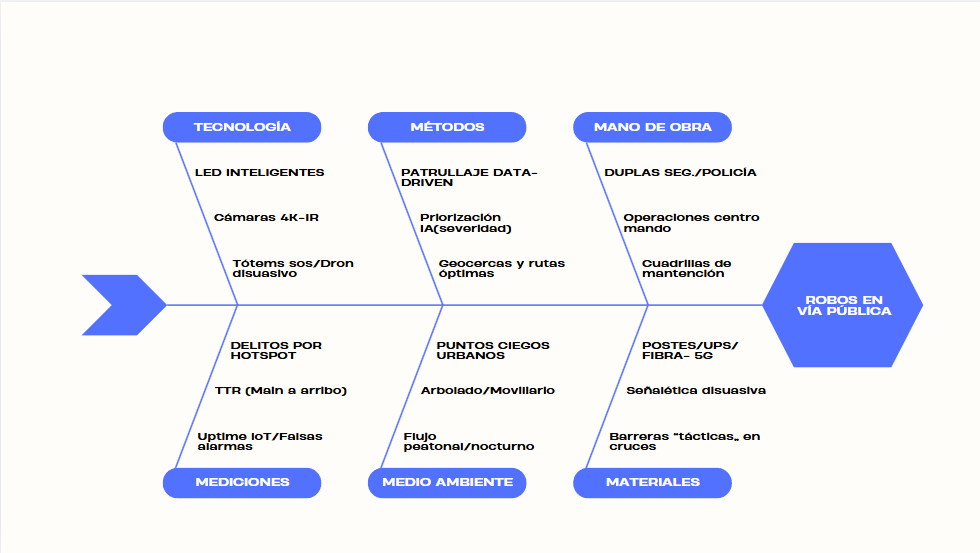
\includegraphics[width=\linewidth, keepaspectratio]{ishikawa_p1.png}
  \caption{Diagrama de Ishikawa del problema \textit{Robos en vía pública}.}
  \label{fig:ishikawa-seguridad}
\end{figure}
\fi


\end{document}
